\documentclass[titlepage, 12pt]{article}

\usepackage{framed}
\usepackage{enumitem}
\usepackage{geometry}
\geometry{
  letterpaper,
  margin=1in,
}

\usepackage{graphicx}
\graphicspath{{.}}
\usepackage{float}

\title{SE 2XB3 Group 4 Report 2}
\author{
  Huang, Kehao \\
  400235182 \\
  \texttt{huangk53@mcmaster.ca} \\
  L01
  \and
  Jiao, Anhao \\
  400251837 \\
  \texttt{jiaoa3@mcmaster.ca} \\
  L01
  \and
  Ye, Xunzhou \\
  400268576 \\
  \texttt{yex33@mcmaster.ca} \\
  L01
}
\date{\today}

\begin{document}
\maketitle{}

\newpage{}

\section{Timeing Data}

\subsection{Analysis of $f(n)$}

$f(n)$ is determined to be growing in the order of $\mathcal{O}(n)$. We started by 
plotting $f(n)$ on a x-y plane and observed a graph similar to that of 
a linear function. We formed our speculation on $f(n)$ being linear. A 
linear regression on the data set was then attempted to further 
investigate. The resulting coefficient of determination is 0.9992, 
indicating that there is a high chance that $f(n)$ is indeed a linear 
function. To confirm our guesses, we plotted a log-log graph for $f(n)$ 
and performed linear regression on the plot. Both the slope of the trend 
line and the $R^{2}$ value were approximately 0.9994. This 
is strong evidence that $f(n)$ grows in the order of $\mathcal{O}(n)$.

\begin{figure}[h]
    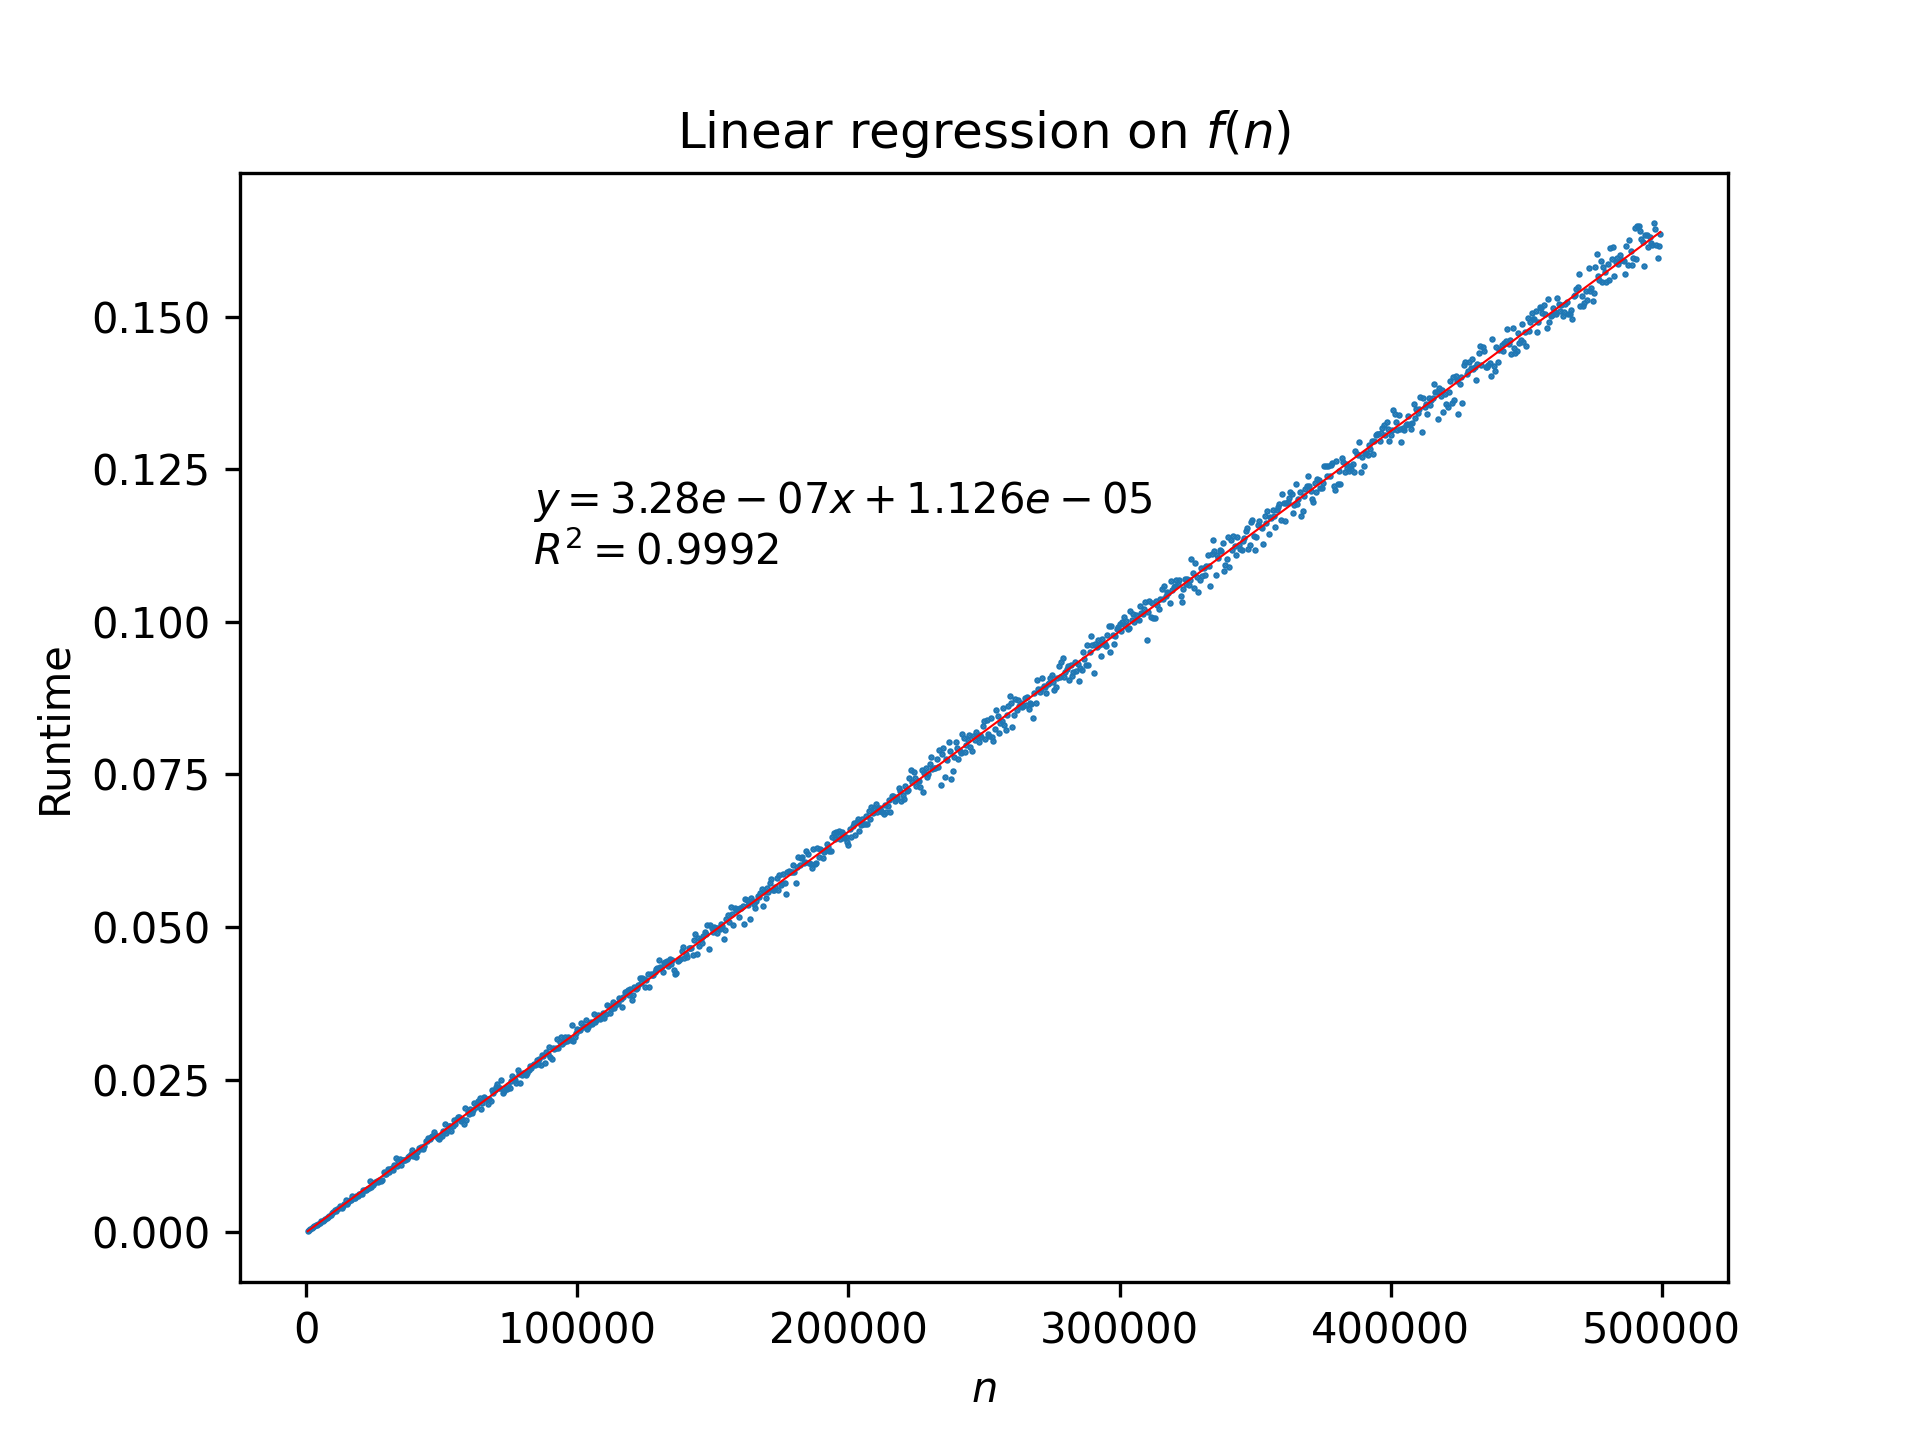
\includegraphics[width=\linewidth]{fn-linreg.png}
    \caption{f(n) linear regression}
\end{figure}
\begin{figure}[h]
    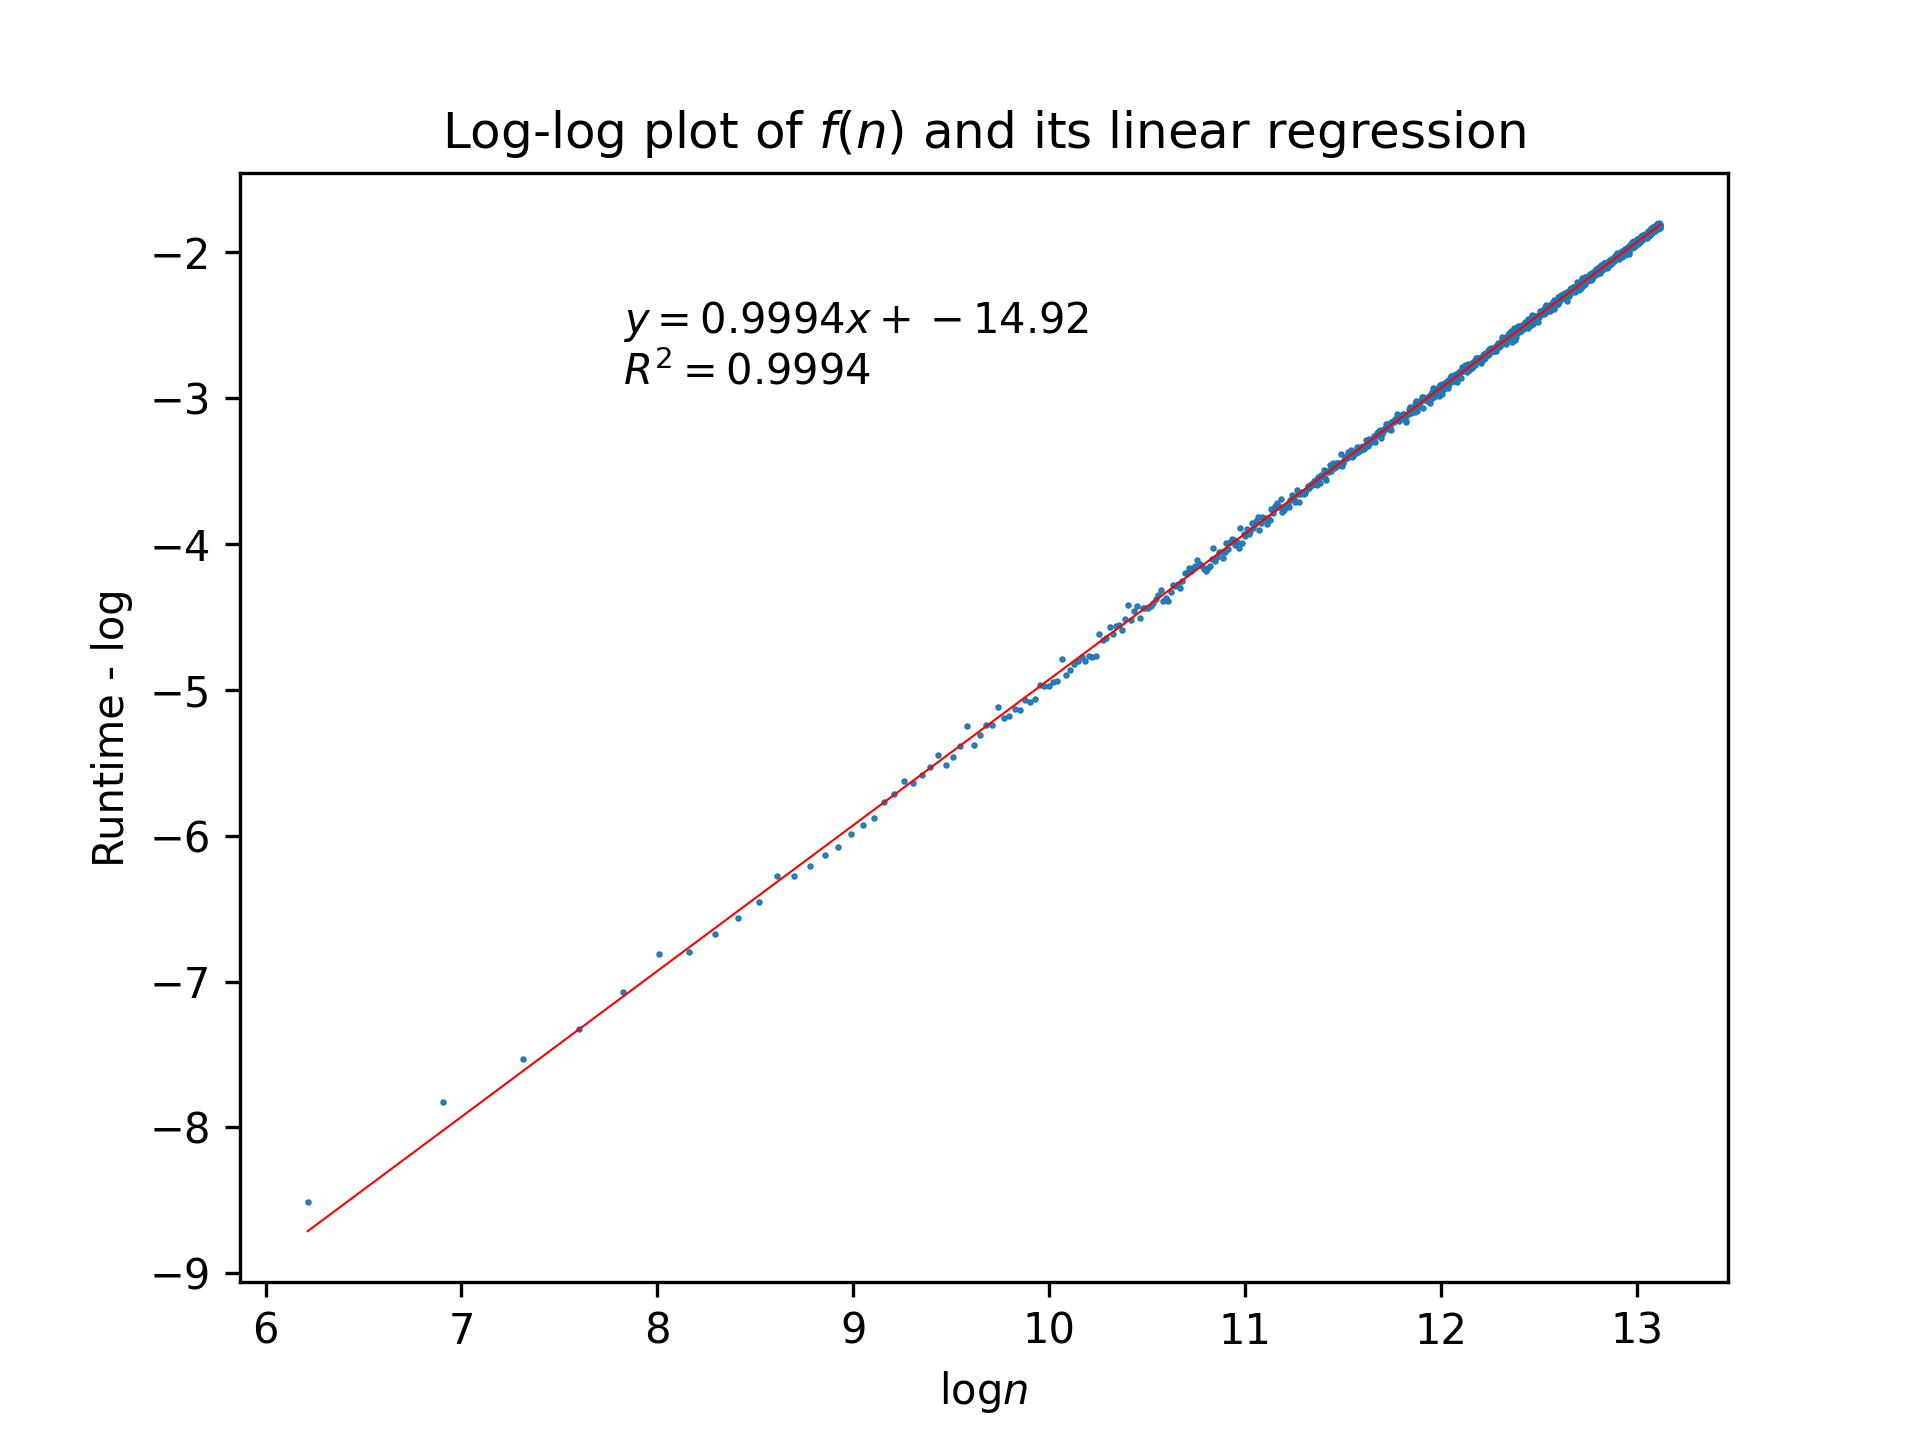
\includegraphics[width=\linewidth]{fn-log-linreg.png}
    \caption{f(n) log linear regression}
\end{figure}

\subsection{Analysis of $g(n)$}
By observing the graph of $g(n)$, our guess on the order of growth was polynomial 
or power. After applying the fitting line and constructed $R^{2}$ value, we found 
that the polynomial function with power of 3 fit the dots the most. However, 
the coefficient of $x^{3}$ is relatively smaller than the coefficient of $x^{2}$. To 
confirm our hypothesis on the growth order, we plotted the log graph and resulted 
in a linear regression with 2.8548 as the coefficient of $x$. Because there were 
nly 43 pairs of data were given for $g(n)$, so the insufficient amount of data 
ould cause the difference between 2.8548 and 3(the expected growth rate). 
Overall, with the finite given date set, we concluded that $g(n)$ has a growth 
order of $\mathcal{O}(x^{3})$

\subsection{Analysis of $h(n)$}
After plotting the $h(n)$ data set into the graph, our first intuition about the 
type of growth was linear. However, by the visual contrast with the $h(n)$ (figureh(n)1), 
we all thought that the fitting line bended too much as a linear function. 
Therefore, we made the second graph which plotted with $log(n)$ and $log(runtime)$ 
(figureh(n)2), as the x-axis and the y-axis respectively. Then, we analyzed the 
coefficient of the term that has the highest power($x$). Compared to 1, the 
oefficient 1.1069 is off by quite a bit. At this point we were uncertain about 
the intuition we had at the beginning. Because the coefficient is larger than 1 
which means it grows faster than linear, however, not as much as polynomial, 
exponential or power functions. At this point, we doubted that it could be $nlog(n)$ 
form. Last but not least, we divided the runtime($nlog(n)$) by its number($n$) and we 
got the figure(h(n)3). Our assumption was right and the graph fits as a log function. 
In conclusion, the $h(n)$ grows in the order of $\mathcal{O}(nlog(n))$

\end{document}